\documentclass{article}

% Language setting
% Replace `english' with e.g. `spanish' to change the document language
\usepackage[french]{babel}

% Set page size and margins
% Replace `letterpaper' with `a4paper' for UK/EU standard size
\usepackage[letterpaper,top=2cm,bottom=2cm,left=3cm,right=3cm,marginparwidth=1.75cm]{geometry}

% Useful packages
\usepackage{amsmath}
\usepackage{graphicx}
\usepackage[colorlinks=true, allcolors=blue]{hyperref}

\title{Journal de bord - TowerDefense}
\author{CHADEVILLE - TECHER}

\begin{document}
\maketitle


\section{Introduction}

Dans le cadre de notre formation, module Computer Science, il nous est demandé de réaliser, en C++, une version simplifiée du Tower Defense, jeu emblématique des années 90. Le travail doit être mené en groupe de 2 ou 3 étudiants. Notre équipe est composée d’Alexandre TECHER et d’Enzo CHADEVILLE.

Ce document sera mis à jour régulièrement afin de suivre l’avancement du projet de manière bimensuelle. Il présentera nos idées, nos réussites, nos échecs ainsi que nos tentatives d’amélioration. Il fera office de journal de bord et constituera une trace du développement du projet.  

\section{Contraintes}
Le projet comporte plusieurs contraintes imposées par notre enseignant :

\begin{itemize}
\item La carte de jeu doit contenir au moins un ou deux chemins possibles, ainsi que des zones ouvertes permettant le placement de tours
\item Le terrain doit être conçu de manière à ce que le joueur puisse réfléchir à des stratégies visant à allonger le parcours des ennemis
\item Si tous les chemins menant aux ressources sont bloqués, alors les ennemis ignorent les tourelles
\item Le programme doit être développé en programmation orientée objet (Ennemis, Tours, Carte, ...).
\item Le programme doit inclure un algorithme de « chemin le plus court »
\end{itemize}

\newpage

\section{Objectifs du projet}

\subsection{Mécanique de gameplay}


\paragraph{}
Le jeu comporte une carte (map) sur laquelle le joueur pourra créer des tours afin d'éliminer les ennemis qui apparaissent.

La map, de forme rectangulaire et de dimensions $(X, Y)$, est divisée en trois zones :

\begin{itemize}
    \item Une zone d'apparition des ennemis ;
    \item Une zone dans laquelle le joueur peut poser ses tours ;
    \item Une zone de fin de parcours pour les ennemis.
\end{itemize}

Un exemple de la disposition des zones sur la carte est présenté à la figure~\ref{fig:zones_map}.

\begin{figure}[!h]
\centering
    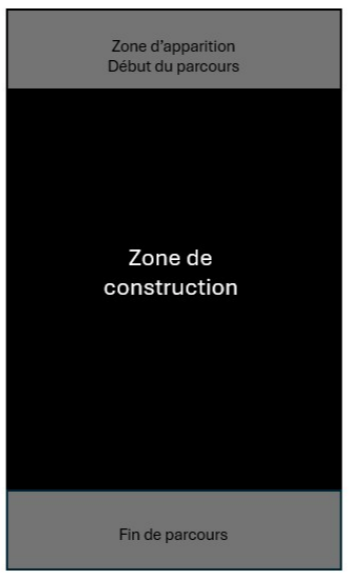
\includegraphics[width=0.22\textwidth]{figs/map.png}
    \caption{Disposition des zones sur la carte.}
    \label{fig:zones_map}
\end{figure}


\paragraph{}
Les ennemis apparaissent à une position aléatoire dans la zone de départ et doivent atteindre la fin du parcours en utilisant un algorithme de type "chemin le plus court".

Si un ennemi atteint la fin du parcours, le joueur perdra des points de vie.

Pour se défendre, le joueur peut placer des tours qui infligent des dégâts et peuvent également influencer le chemin des ennemis.

La figure~\ref{fig:tours_ennemis} illustre l'impact du placement des tours sur la trajectoire des ennemis.

\begin{figure}[!h]
\centering
    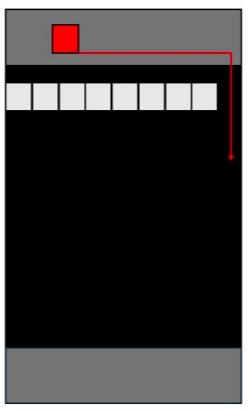
\includegraphics[width=0.22\textwidth]{figs/gpmap.png}
    \caption{Placement des tours pour dévier le chemin des ennemis.}
    \label{fig:tours_ennemis}
\end{figure}

Ainsi, plus le joueur place judicieusement ses tours, plus le chemin des ennemis s'allongera, augmentant les chances de les éliminer avant qu'ils n'atteignent la fin de la carte.


\newpage

\subsection{Inspiration}

Pour notre Tower Defense, nous allons nous inspiré (au niveau du gameplay et une partie de l'HUD) de Tower Wars: StarCraft 2, un mode personnalisé créé dans l’éditeur de cartes de Starcraft 2. 

Nous nous inspirons également de Age Of empire pour son HUD des ressources.

\section{Planning prévisionnel}

Semaines 36-37 :
\begin{itemize}
\item Mise en commun des idées et accord sur le résultat souhaité.
\item Rédaction d’un cahier des charges.
\item Apprentissage de GitHub, \LaTeX{} et découverte de SFML.
\item Mise en place d’une ébauche du squelette du programme.
\item Début de la création du jeu.
\end{itemize}

Semaines 38-41 :
\begin{itemize}
\item Mise en place des différents outils de travail (GitHub, \LaTeX).
\item Affichage d’une fenêtre SFML et début d’un premier prototype de jeu.
\end{itemize}

Semaines 42-45 :
\begin{itemize}
\item Finalisation d’une version minimaliste du jeu.
\item Début de la création des menus et de la gestion des ressources.
\end{itemize}

Semaines 46-48 :
\begin{itemize}
\item Finalisation de la gestion des ressources et menus fonctionnels.
\item Début de la mise en place de la direction artistique (sprites).
\item Consolidation de l’équilibrage du jeu.
\end{itemize}

Semaines 49-52 :
\begin{itemize}
\item Finalisation de la direction artistique.
\item Équilibrage conforme à nos attentes.
\item Optimisation du programme.
\item Création d’un menu de jeu complet.
\item Démo jouable du Tower Defense.
\end{itemize}

\end{document}